%---------------------------------------------------------------------------------------------------------------%
\section{Fase --- A}
%---------------------------------------------------------------------------------------------------------------%

Nesta fase, requer-se que se especifique uma MIB com que implemente dois grupos:
um grupo (\texttt{unpredictableParam}) que conterá os parâmetros de
funcionamento do servidor, nomeadamente o rácio de refrescamento (\texttt{R}),
o número de entrada na tabela (\texttt{N}), o tamanho dos dígitos hexadecimais
(\texttt{D}) e, adicionalmente, um objeto escalar de cariz especial, do tipo
\emph{string} e com apenas permissões de escrita, para a operação do
\emph{reset} do agente; outro grupo (\texttt{unpredictableTable}) com a tabela
de \texttt{N} números aleatórios, onde a mesma deve incluir apenas duas colunas,
uma para o índice de entrada (chave da tabela) e outra para um número aleatório
(sequência de \texttt{D} dígitos hexadecimais).

Procedeu-se de seguida ao desenho da MIB, segundo uma árvore do OID's, onde se
decidiu que o módulo da MIB, no âmbito deste trabalho, ficasse abaixo do nodo
\emph{experimental} com o identificador 99. Adicionalmente, e para o ficheiro
ficar \emph{bem formado}, adicionou-se dois \texttt{OBJECT-GROUP} para os grupos
mencionados acima, uma vez que, cada objeto numa MIB deve ser incluído pelo
menos numa definição de grupo, seja ela, \texttt{OBJECT-GROUP} ou
\texttt{NOTIFICATION-GROUP} (RFC2580 §3.1 and §4.1). A hierarquia da árvore fica
como está na \emph{Figura~\ref{fig:fasea:arvoreoids}}. 


\begin{center}
 	
	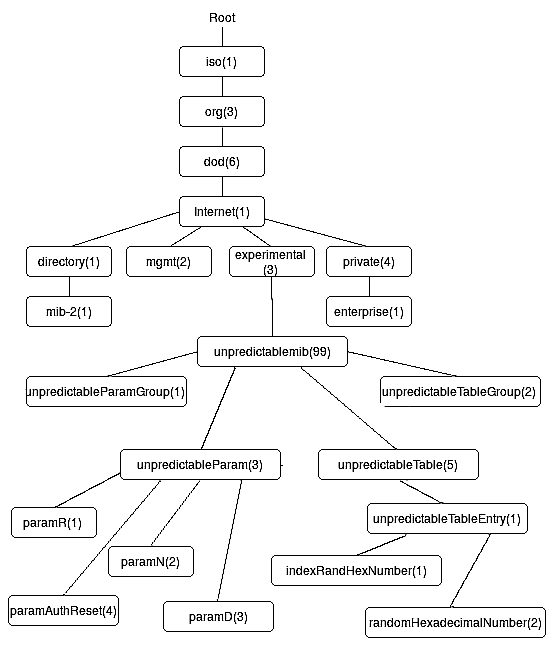
\includegraphics[scale=0.75,keepaspectratio]{resources/images/faseA/arvoreOID.png}
 	\captionsetup{type=figure, width=0.8\linewidth}
	\caption{Árvore de OIDs}
\label{fig:fasea:arvoreoids} 
\end{center}

\newpage

Em seguida procedeu-se à redação da MIB, com a consequente validação no software
\emph{MibDesigner}. Em primeiro lugar definiram as convenções textuais e tipos
de objeto a importar. Como foi anteriormente se disse, é necessário implementar
dois objetos do tipo \emph{string}: o parâmetro de autenticação para
\emph{reset} no agente e o número hexadecimal. Assim, decidiu-se importar
a convenção textual \emph{DisplayString} e o tipo \texttt{OBJECT-GROUP} (este
último justificado anteriormente). A secção de \emph{imports} pode-se ver na
figura \emph{FIgura~\ref{fig:fasea:imports}}.  

\begin{center}
 	
 	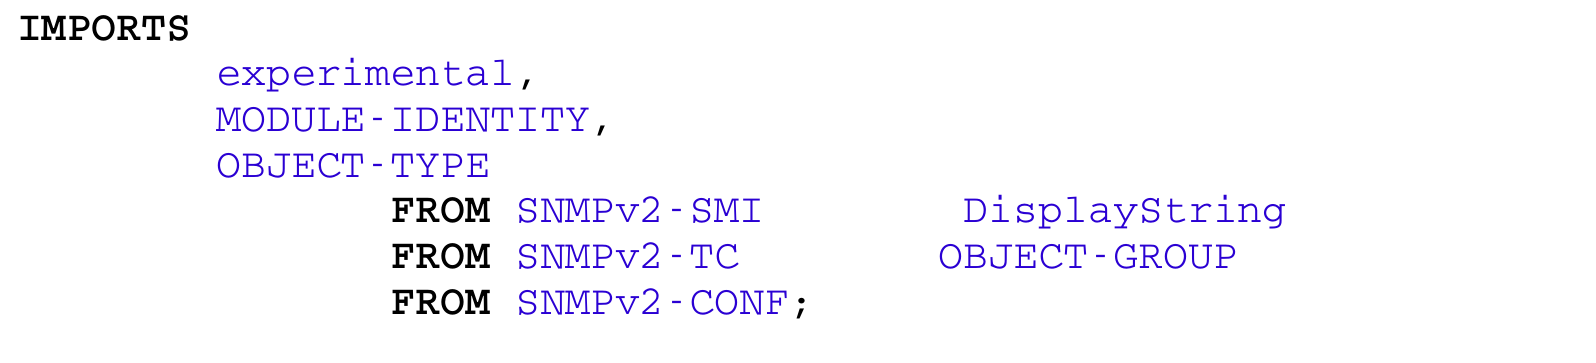
\includegraphics[width=\textwidth,height=\textheight,keepaspectratio]{resources/images/faseA/mib/imports.png}
 	\captionsetup{type=figure, width=0.8\linewidth}
	\caption{\emph{Imports} }
\label{fig:fasea:imports} 
\end{center}

\newpage

Definiu-se, também o módulo da MIB, com o nome
\texttt{unpredictableMIB}. Este tem, para além do número identificador uma série
de informações sobre quem fez o módulo, contatos, descrição e afins. A sua
definição pode ser verificada na \emph{Figura~\ref{fig:fasea:modulo}}. 

\begin{center}
 	
 	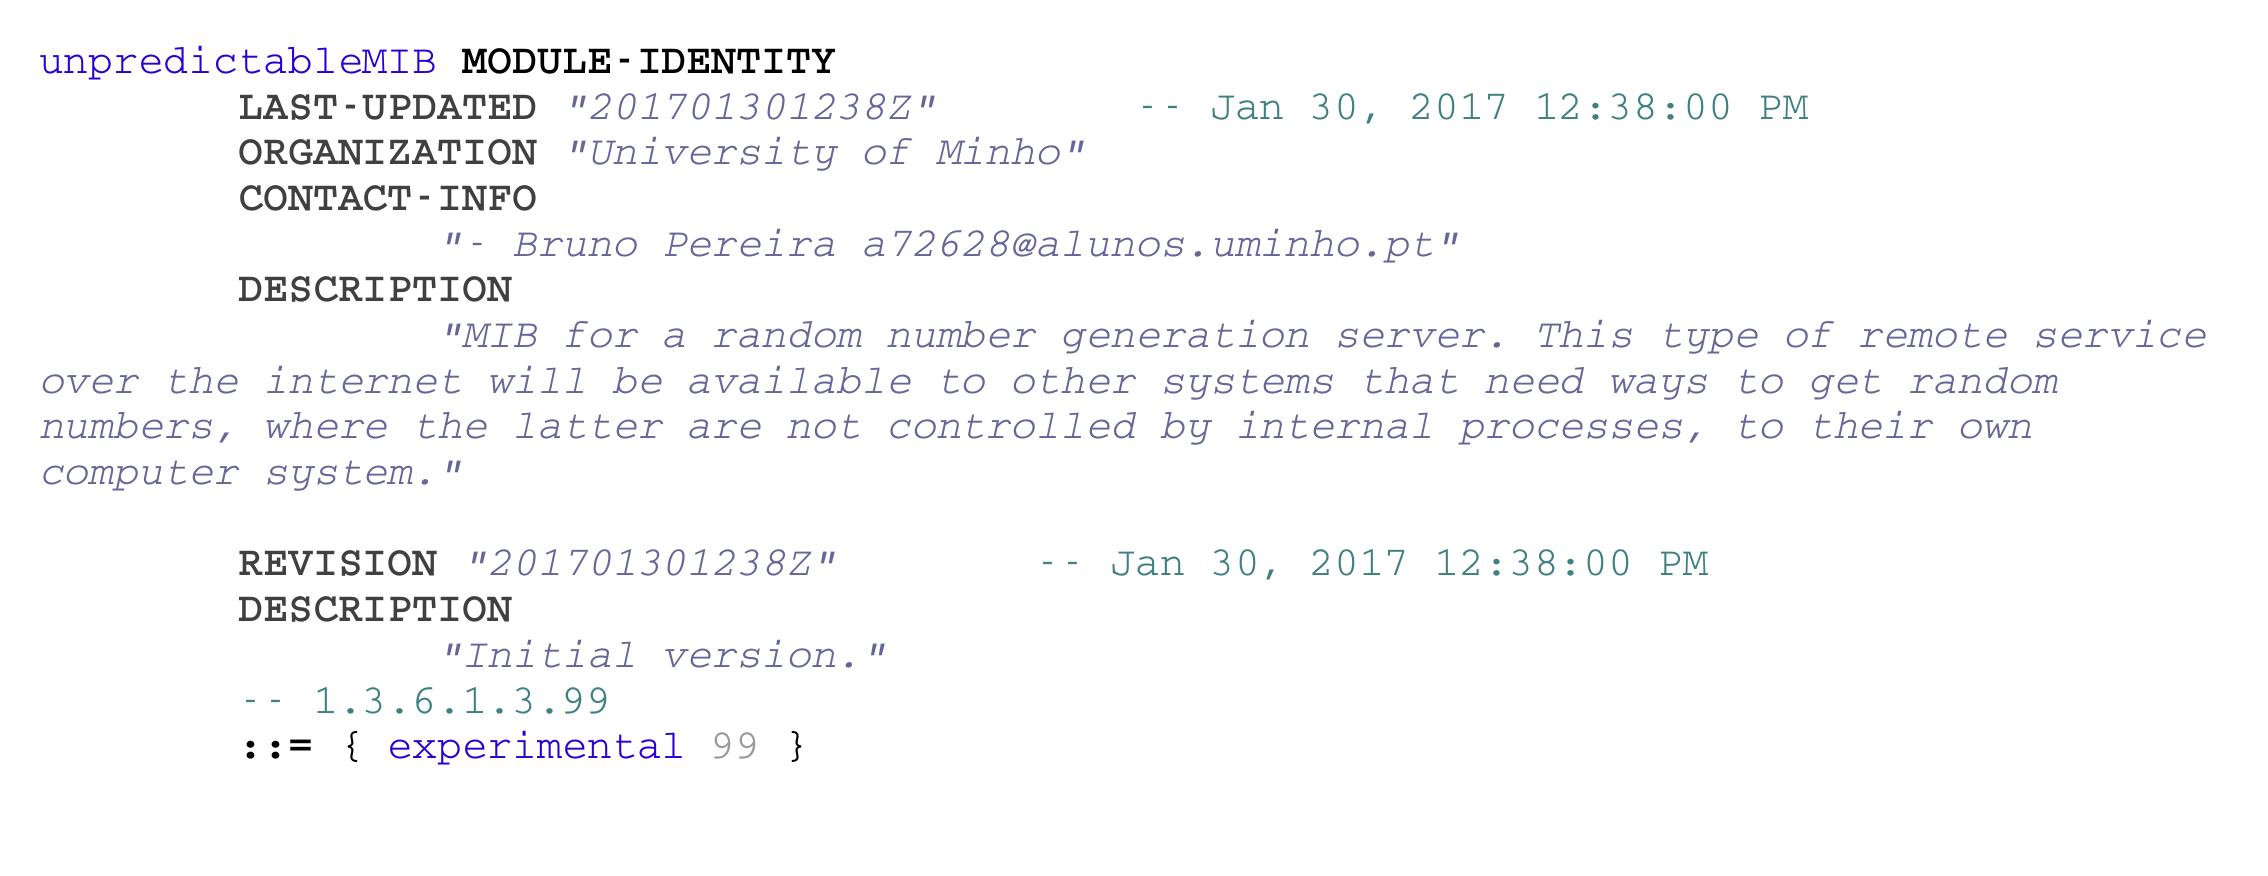
\includegraphics[width=\textwidth,height=\textheight,keepaspectratio]{resources/images/faseA/mib/modulo.png}
 	\captionsetup{type=figure, width=0.8\linewidth}
	\caption{Módulo \texttt{unpredictableMIB} }
\label{fig:fasea:modulo} 
\end{center}



Seguidamente, definiram os \texttt{OBJECT-GROUP} incluindo os objetos em cada
grupo, respetivamente. Note-se que, a ordem porque está esta declaração, tem
o intuito de declarar os grupos, como protótipos dos grupos segundo a sua
propriedade, neste caso como devem ser implementados em grupo. Adicionalmente,
criou-se um \texttt{OBJECT-IDENTIFIER} para o grupo \texttt{unpredictableParam}.
Note-se que não se fez o mesmo para o grupo \texttt{unpredictableTable} porque,
como se poderá ver em seguida, não faz sentido adicionar um nível intermédio na
árvore de OID's, uma vez que a definição do objeto tabela é um grupo.

\begin{center}
 	
 	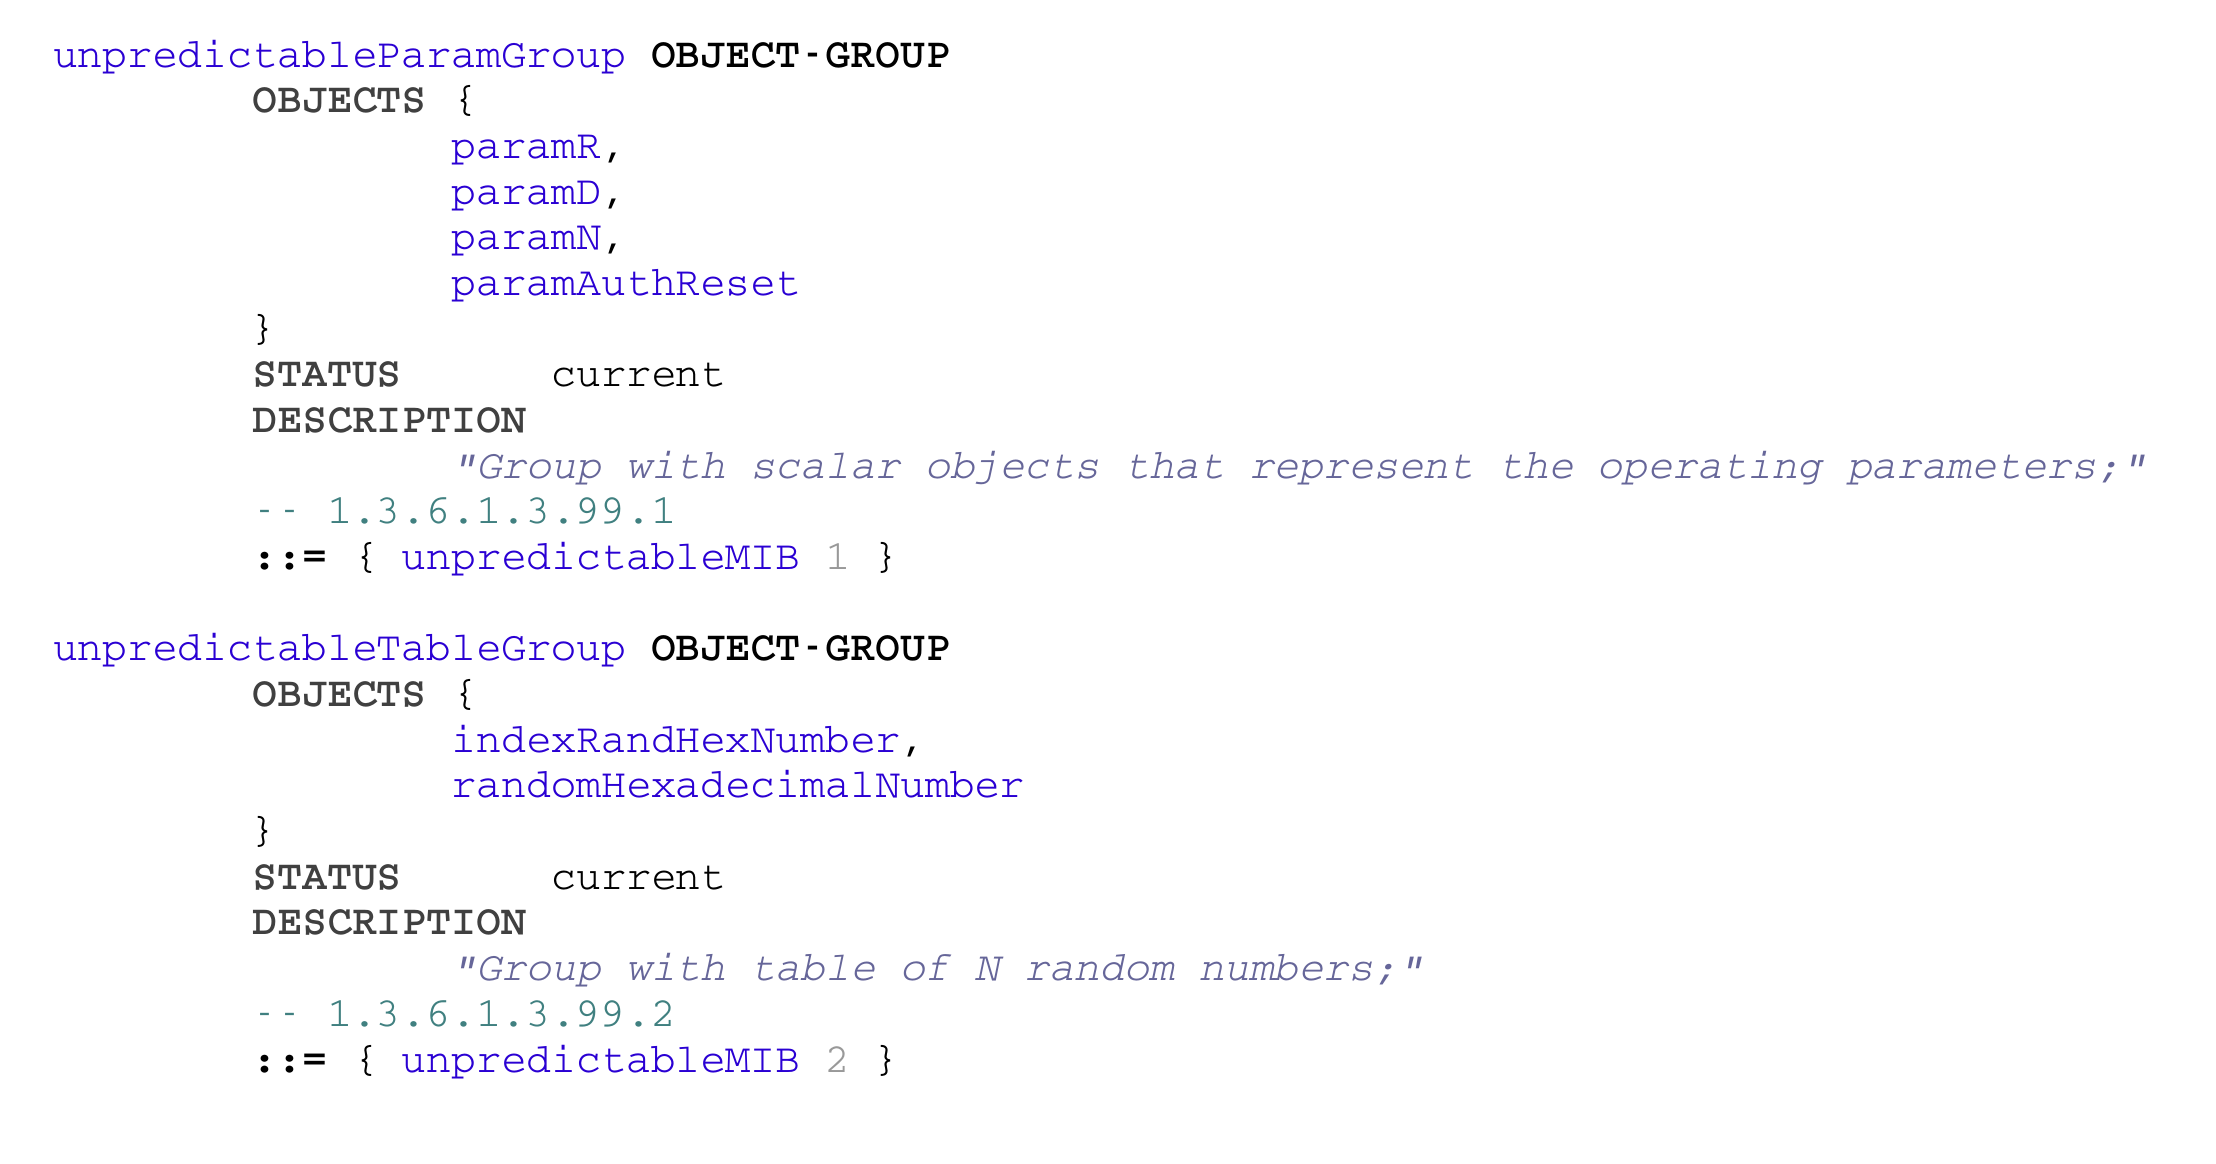
\includegraphics[width=\textwidth,height=\textheight,keepaspectratio]{resources/images/faseA/mib/groups.png}
 	\captionsetup{type=figure, width=0.8\linewidth}
	\caption{Grupos necessários}
\label{fig:fasea:groups} 
\end{center}

\newpage

\begin{center}
 	
 	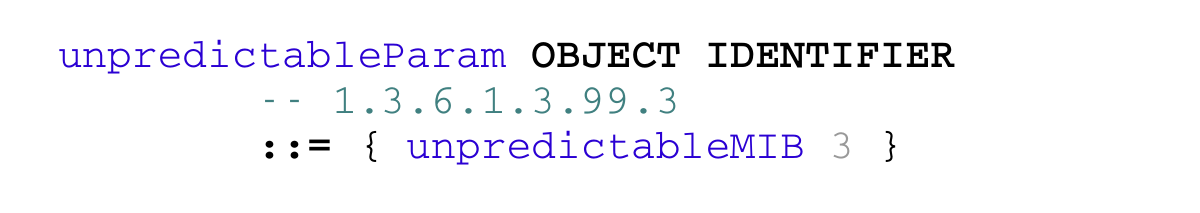
\includegraphics[width=\textwidth,height=\textheight,keepaspectratio]{resources/images/faseA/mib/scalars/groupid.png}
 	\captionsetup{type=figure, width=0.8\linewidth}
	\caption{Definição do identificador de grupo de escalares}
\label{fig:fasea:groupid} 
\end{center}

Depois adicionaram-se os escalares para os parâmetros de funcionamento do
agente. Estes objetos são todos \emph{read-only}, exceto o \emph{paramAuthReset}
que é \emph{read-write}. Note-se que o \emph{MibDesigner} não possuía a opção
\emph{write-only}, no entanto, estas definições foram depois refinadas ao nível
do código do agente, seja da definição da VACM, seja no acesso do objeto.


\begin{center}
 	
 	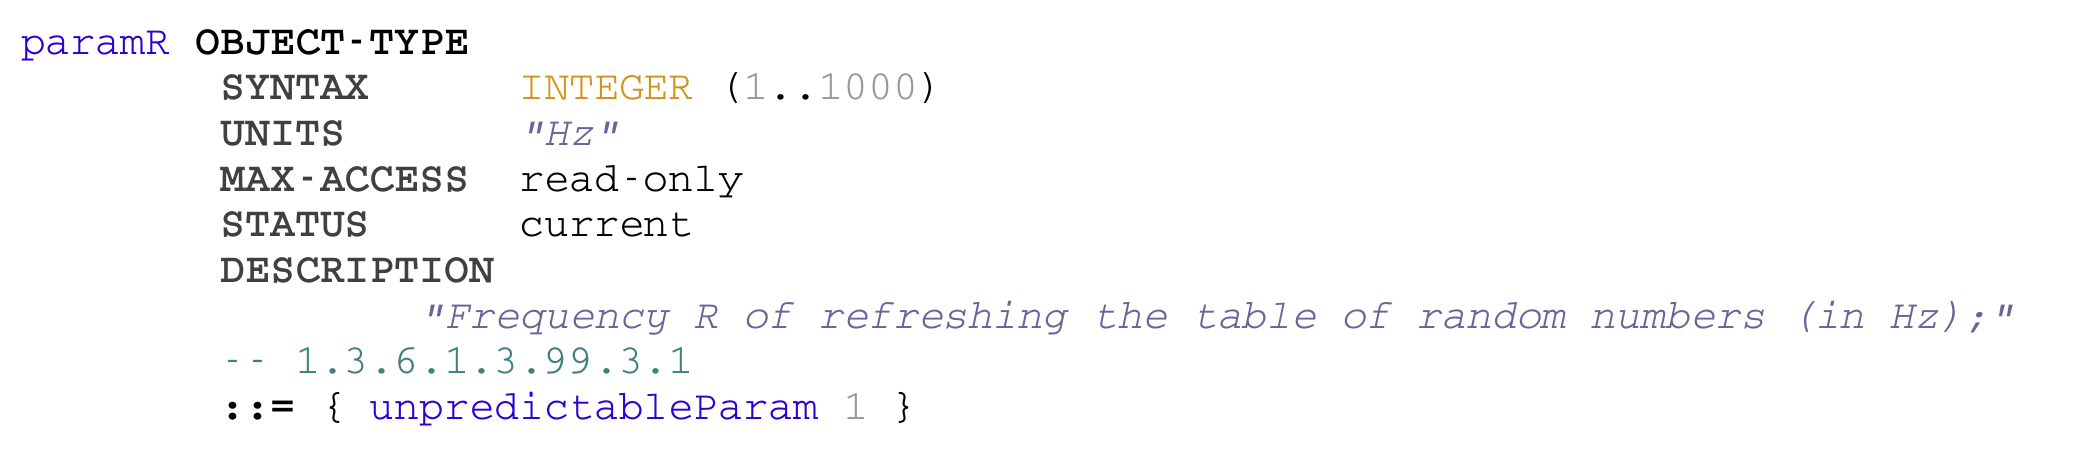
\includegraphics[width=\textwidth,height=\textheight,keepaspectratio]{resources/images/faseA/mib/scalars/paramR.png}
 	\captionsetup{type=figure, width=0.8\linewidth}
	\caption{Escalar para refrescamento (parâmetro R)}
\label{fig:fasea:} 
\end{center}

\begin{center}
 	
 	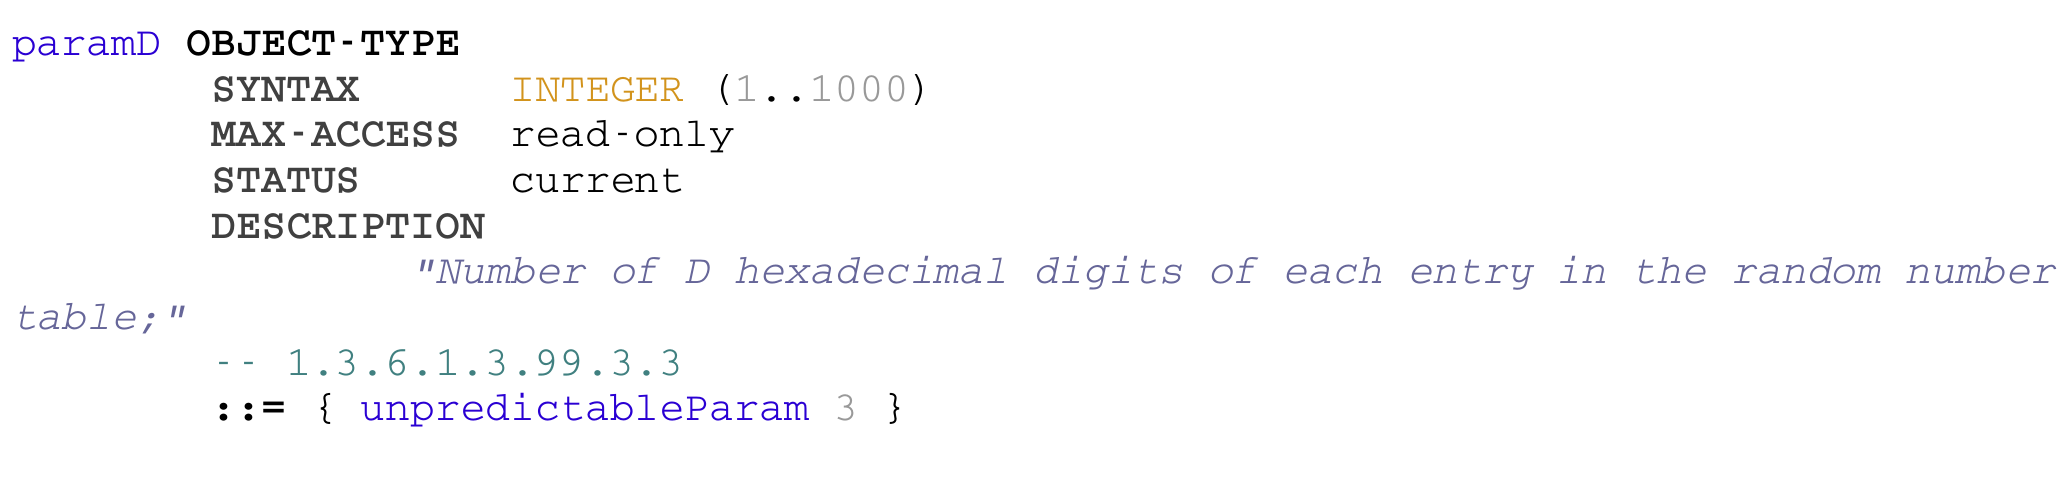
\includegraphics[width=\textwidth,height=\textheight,keepaspectratio]{resources/images/faseA/mib/scalars/paramD.png}
 	\captionsetup{type=figure, width=0.8\linewidth}
	\caption{Escalar para número de dígitos hexadecimais (parâmetro D)}
\label{fig:fasea:} 
\end{center}

\begin{center}
 	
 	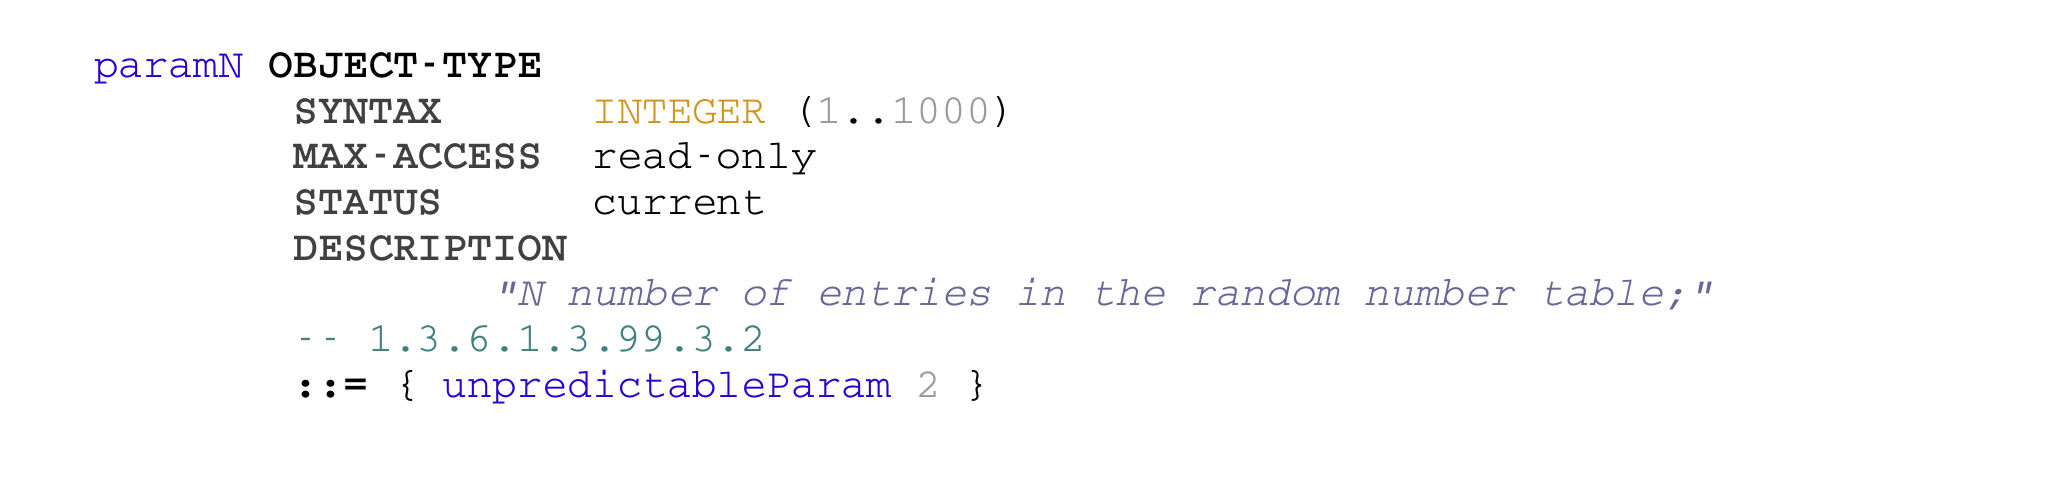
\includegraphics[width=\textwidth,height=\textheight,keepaspectratio]{resources/images/faseA/mib/scalars/paramN.png}
 	\captionsetup{type=figure, width=0.8\linewidth}
	\caption{Escalar para número de linhas da tabela (parâmetro N)}
\label{fig:fasea:} 
\end{center}

\begin{center}
 	
 	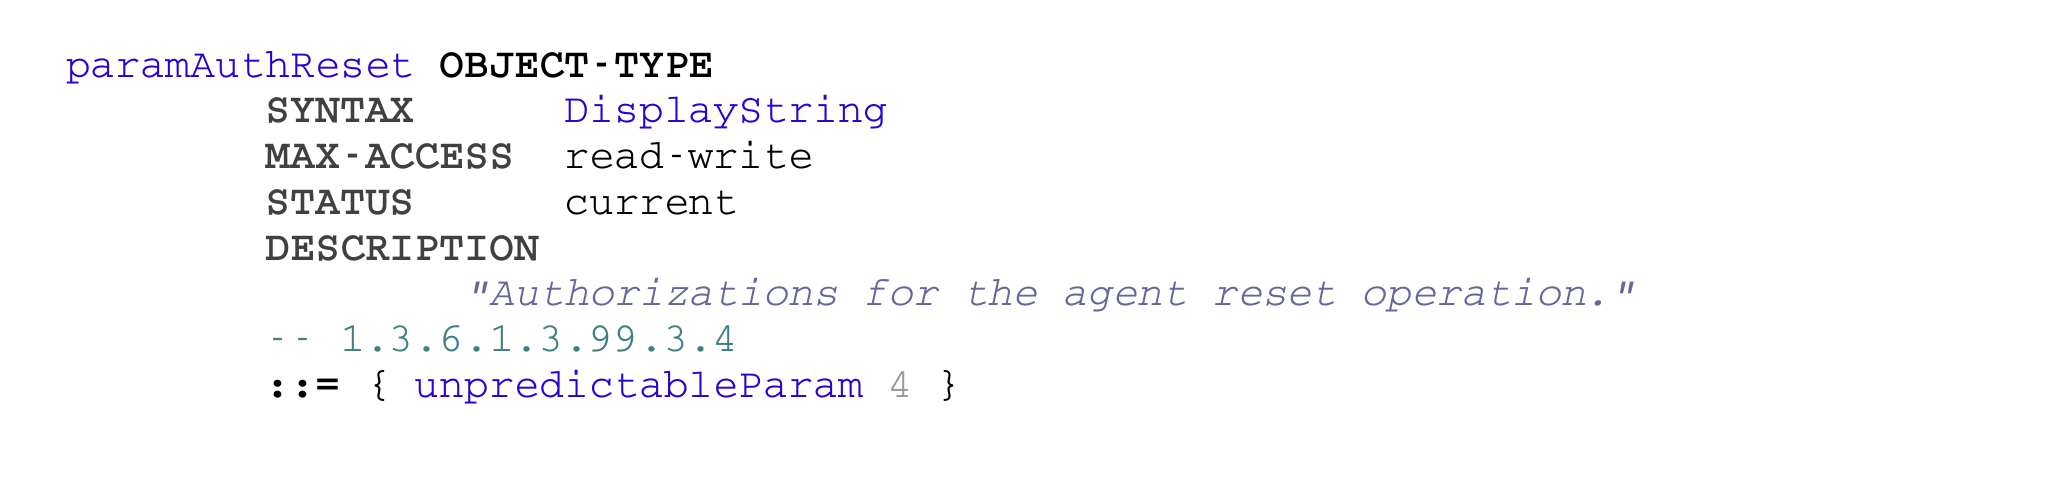
\includegraphics[width=\textwidth,height=\textheight,keepaspectratio]{resources/images/faseA/mib/scalars/paramAuthReset.png}
 	\captionsetup{type=figure, width=0.8\linewidth}
	\caption{Escalar para chave de autenticação para \emph{reset} }
\label{fig:fasea:} 
\end{center}

\newpage
A definição da tabela está na figura seguinte, e ficou definida como um
sequência de \emph{UnpredictableTableEntry}, que por sua vez é uma sequência
com o índice da tabela e o número hexadecimal associado. 

\begin{center}
 	
 	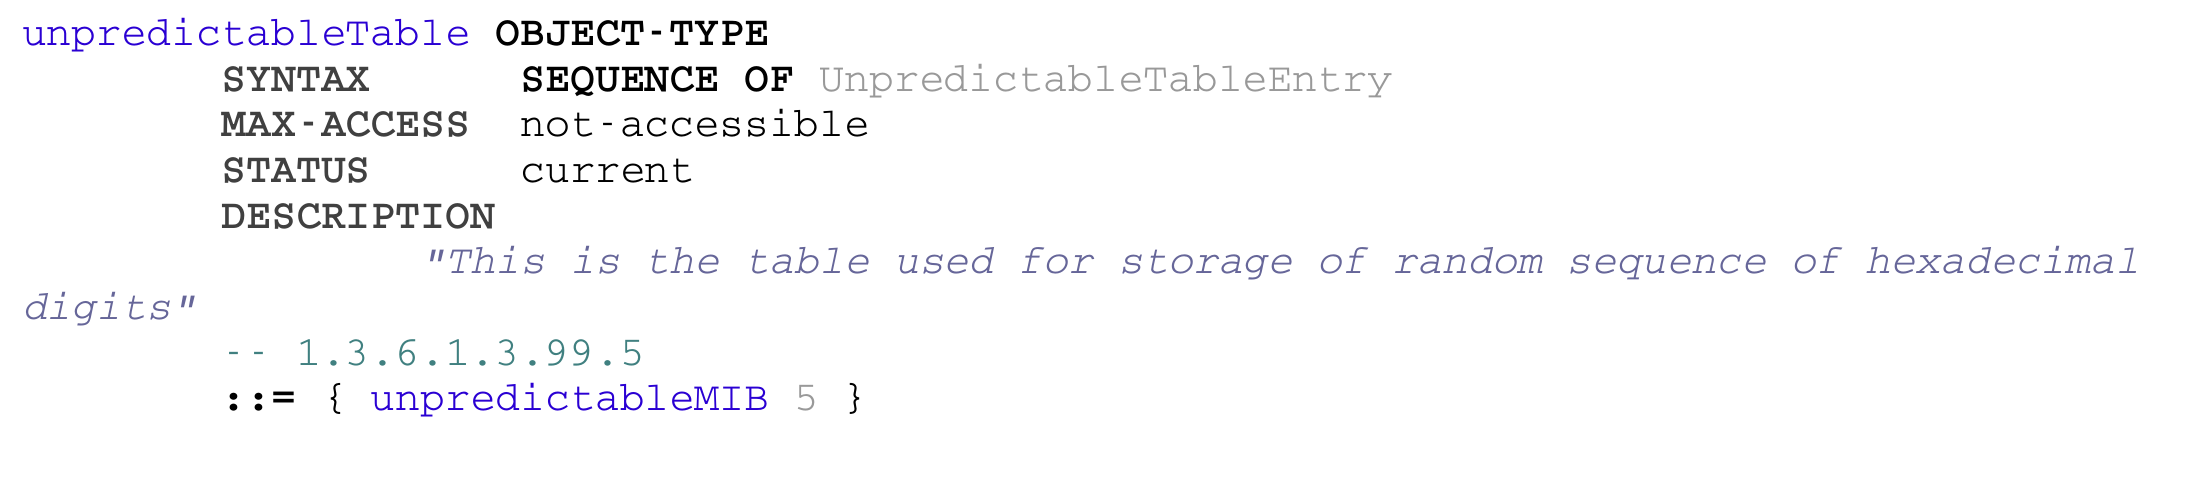
\includegraphics[width=\textwidth,height=\textheight,keepaspectratio]{resources/images/faseA/mib/tables/table.png}
 	\captionsetup{type=figure, width=0.8\linewidth}
	\caption{Identificador de grupo e da tabela}
\label{fig:fasea:} 
\end{center}

\begin{center}
 	
 	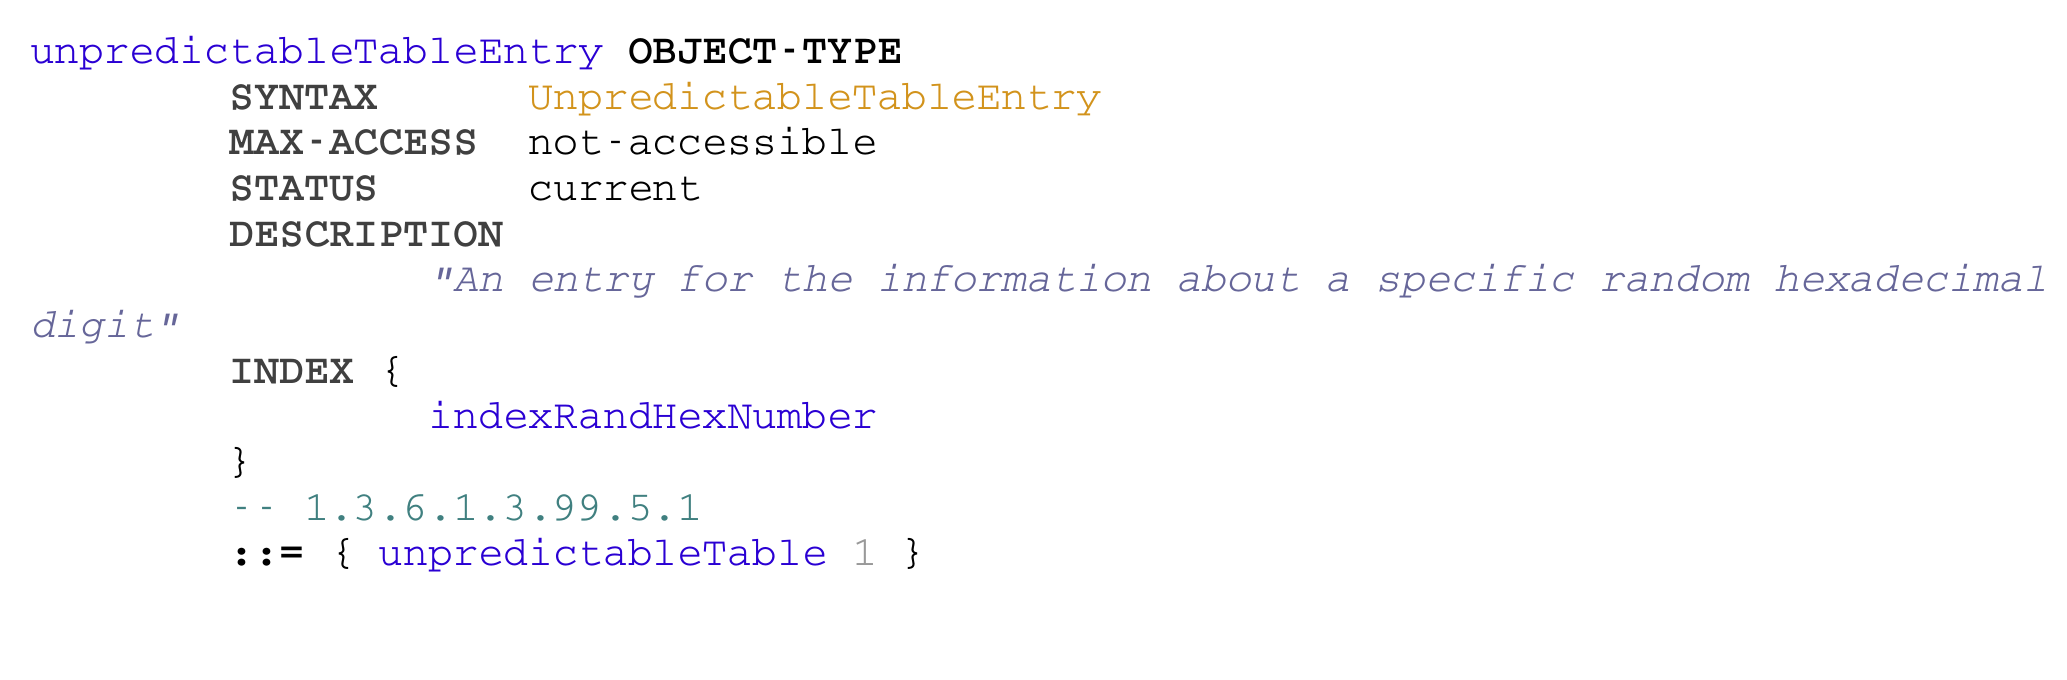
\includegraphics[width=\textwidth,height=\textheight,keepaspectratio]{resources/images/faseA/mib/tables/tableentry.png}
 	\captionsetup{type=figure, width=0.8\linewidth}
	\caption{Definição do tipo da entrada de tabela}
\label{fig:fasea:} 
\end{center}

\newpage
O objeto representativo do índice da tabela, foi definido como \emph{read-only}
e um inteiro entre 1 e 1000. Por sua vez, o objeto representativo do número
hexadecimal foi definido como \emph{read-write}, por motivos aqui já mencionados
e o seu tipo como um \emph{DisplayString}. 

\begin{center}
 	
 	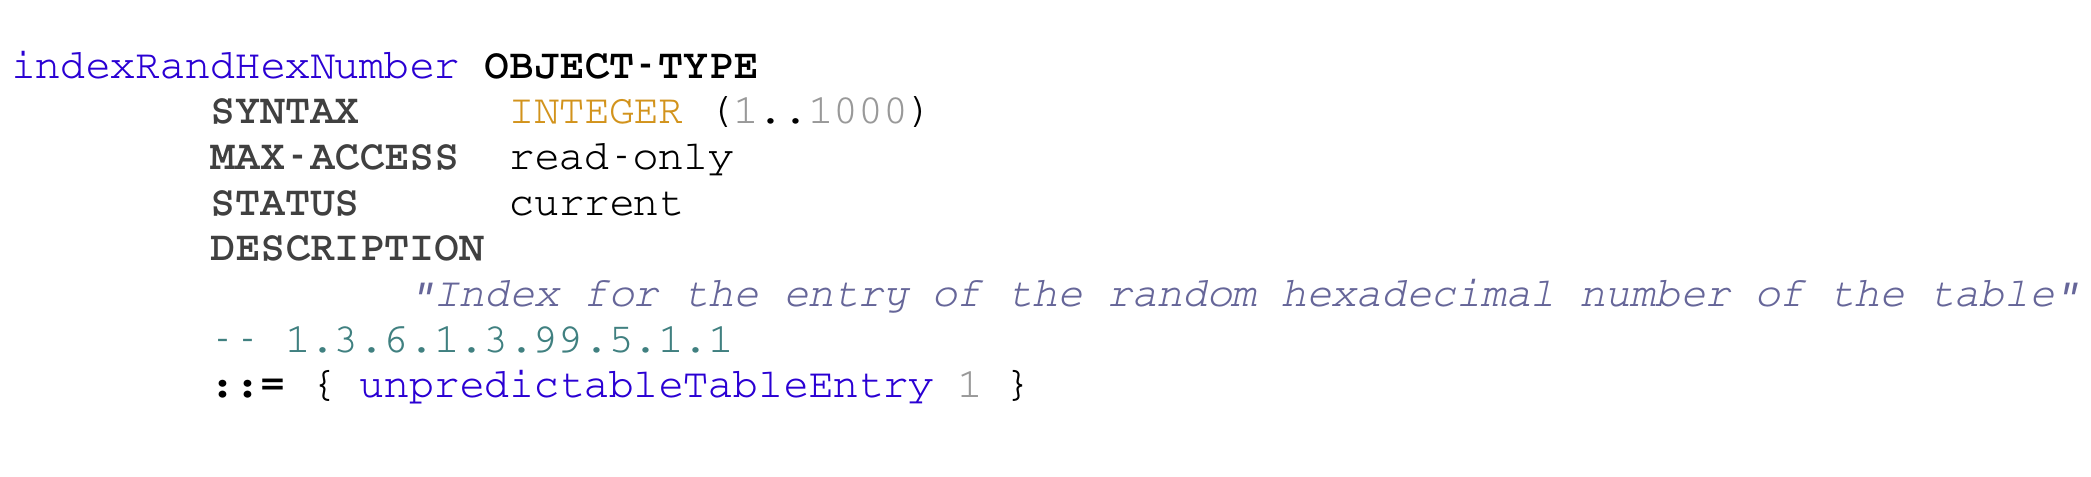
\includegraphics[width=\textwidth,height=\textheight,keepaspectratio]{resources/images/faseA/mib/tables/indextable.png}
 	\captionsetup{type=figure, width=0.8\linewidth}
	\caption{Escalar para indexação da tabela}
\label{fig:fasea:} 
\end{center}

\begin{center}
 	
 	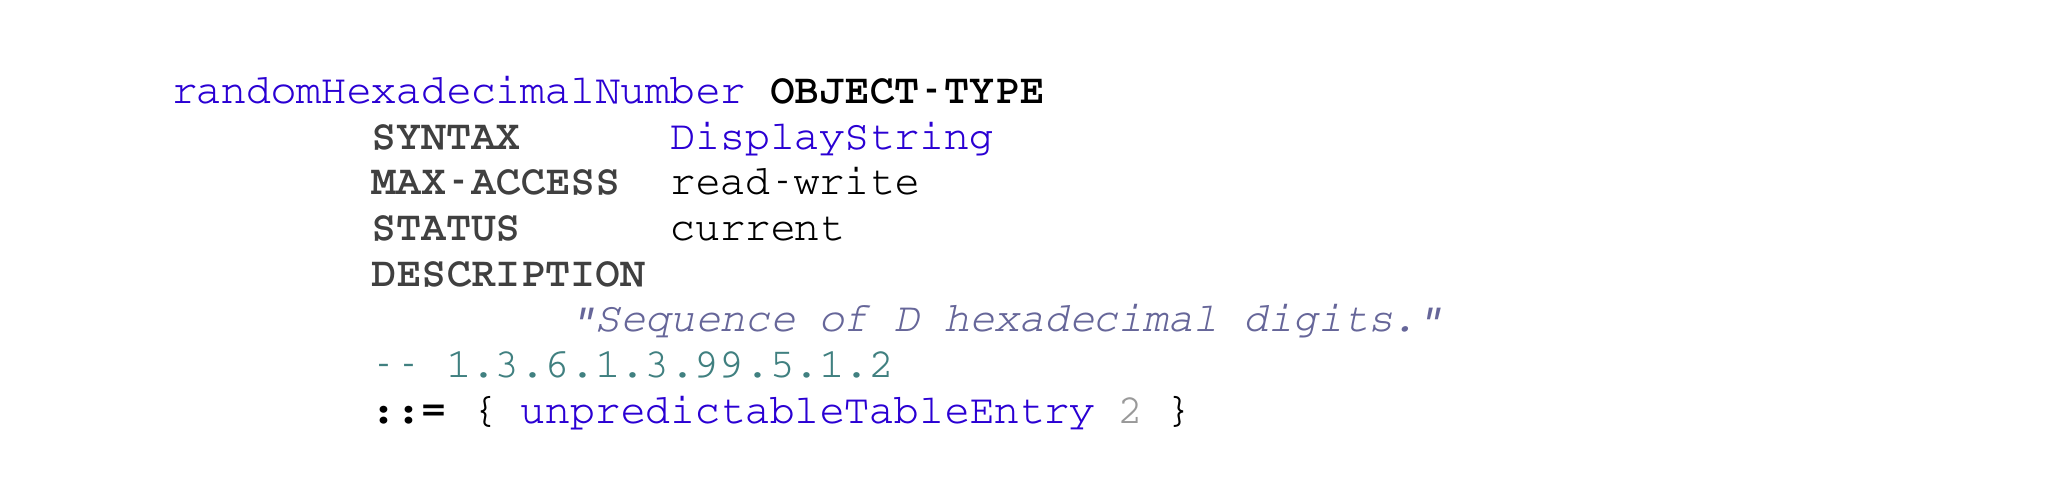
\includegraphics[width=\textwidth,height=\textheight,keepaspectratio]{resources/images/faseA/mib/tables/hexadecimalnumber.png}
 	\captionsetup{type=figure, width=0.8\linewidth}
	\caption{Escalar para representação de um número hexadecimal}
\label{fig:fasea:} 
\end{center}

\begin{center}
 	
 	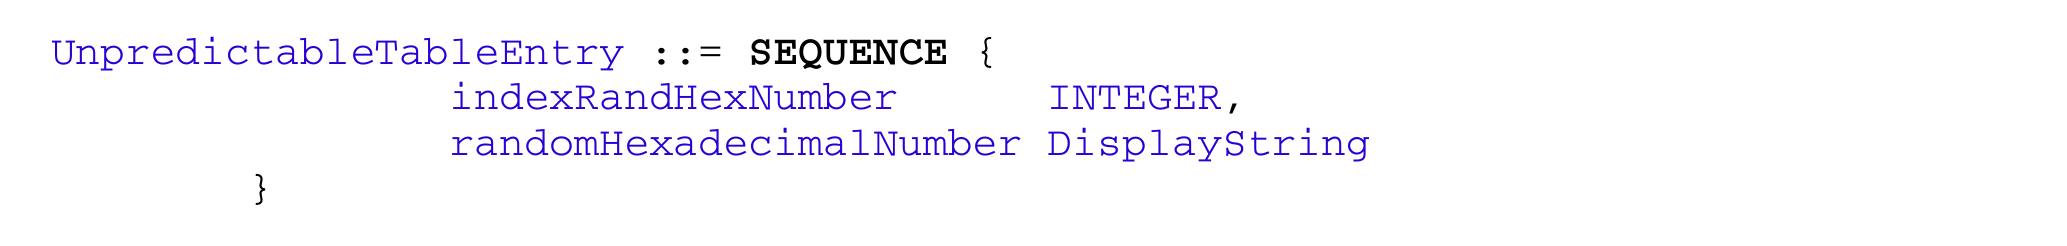
\includegraphics[width=\textwidth,height=\textheight,keepaspectratio]{resources/images/faseA/mib/tables/tableentrydefinition.png}
 	\captionsetup{type=figure, width=0.8\linewidth}
	\caption{Declaração do tipo da entrada da tabela de números hexadecimais}
\label{fig:fasea:} 
\end{center}












